\section{Introduction}
\label{sec:intro}

Supervised machine learning algorithms are trained on data for which correct answers (e.g. classes, predictions) are known in advance, with the goal of producing a system that will subsequently also give the correct answers for new, unseen data. In the context of genetic programming (GP) \cite{koza:book}, this means that we seek to evolve a program that will produce correct outputs when run on any valid inputs, including inputs not encountered during the evolutionary process. That is, we seek programs that {\it generalize} to \textit{unseen test data}. While the challenges of learning generalizing solutions have long been recognized and studied, both in GP (e.g. \cite{1144159, DBLP:conf/gecco/VanneschiG09, Castelli:2010:cec, Goncalves:2015:EuroGP}) and other machine learning algorithms (e.g. \hl{CITE ONE SURVEY}), the challenges in this area have not yet been fully met, and significant  problems remain open.

Another set of long-standing, open research questions in GP concerns the growth of programs over evolutionary time, and the presence of unnecessary code in evolved programs---see, for example, the survey~\cite{silva2012operator}. Such code growth can consume computational resources, slow down the GP search process, and produce programs that are difficult for users to understand or apply.

In this paper we report on work stemming from steps taken to deal with code growth, which then unexpectedly provided substantial and robust benefits with respect to generalization. Specifically, we explore the idea of automatically simplifying evolved programs, originally developed to aid in their analysis and application~\cite{Spector:2014:GECCOcomp}. When using simplification in experiments, we noticed instances in which programs that did not generalize prior to simplification {\it did} generalize {\it after} simplification \cite{Helmuth:2015:dissertation}. In this paper we systematically study the connections between automatic simplification and generalization.

The study presented here was conducted entirely on evolved Push programs, evolved with the PushGP genetic programming system \cite{spector:2002:GPEM}. Push has an unusually permissive syntax, in which any tokens of the language may appear in any order, and all possible programs produce interpretable results. This means that it is particularly easy to automatically simplify Push programs while maintaining program behavior on the training data. To do so, one can remove random tokens from programs, interpret the resulting programs, and compare program behavior before and after such modifications. All of the automatic simplification methods discussed in this paper work this way. 
%In many other GP systems, such as traditional tree-based GP \cite{koza:book}, programs that are modified in this way would often fail to compile or to produce results at all. However, these methods may be applicable to other GP systems.

Automatic simplification was introduced to Push as a tool for making evolved programs easier to understand \cite{Robinson:2001:GPtieus, spector:2002:GPEM}. Smaller solutions have other benefits as well, such as faster runtimes. While it can be applied to any Push program, it has typically been used only after the completion of GP runs, to make solution programs easier to understand without changing their behavior \cite{Spector:2014:GECCOcomp}. It has also been used as a growth-control genetic operator during GP runs, with mixed success \cite{Zhan:2014:GECCOcomp}. Here we consider only post-run simplification, and we focus only on its effects on code size and program generalization.

In the following section we first briefly describe related work on automatic simplification and generalization in GP. We then briefly describe relevant aspects of the Push programming language and our automatic simplification methods. We then describe our experimental design and results, and discuss our conclusions.


\section{Related Work}
\label{sec:related}

%\subsection{Papers about automatic simplification}

Simplification of evolved programs has been used for various reasons in GP, though as far as we know, never explicitly to improve generalization of an evolved solution. Some of the primary uses include making evolved programs easier to understand~\cite{koza:book} and controlling bloat during a run~\cite{1144156, Kinzett:2010:cec, Brameier:2001:TEC, ekart:1999:EA}. %Could remove last one if necessary
Of particular interest is work that uses simplification during a run to reduce overfitting~\cite{Kinzett:2010:cec, hooper:1996:iarGPes}. Additionally, algebraic simplification has been used to combat exponential code growth in geometric semantic genetic programming~\cite{conf/ppsn/MoraglioKJ12}. Unlike our work, most of these methods use algebraic techniques for simplification that cannot change the output of a program on any input, and therefore cannot affect the generalization to unseen data.

Various work has been done to reduce the problems of overfitting in GP~\cite{goncalves:2013:EuroGP, 1144159, DBLP:conf/gecco/VanneschiG09, Castelli:2010:cec, Goncalves:2015:EuroGP}. In other work, an ensemble of symbolic regression datasets were created using bootstrapping~\cite{conf/ppsn/Agapitos12}. Here, the variance of a individual's error on these datasets was used in combination with the error on the original dataset to create a new fitness function. When this new fitness function is used to drive GP, it was shown to produce better generalizing programs.
In \cite{Azad:2011:GECCO} a measure of each individual's variance of output values (referred to as smoothness) is used in a modified version of tournament selection. This scheme was shown to produce better generalizing programs on symbolic regression problems.

Relations between program size and and generalization have been studied previously. Many of these studies have been conducted in the context of tree based genetic programming, which has an idiosyncratic tendency to produce program ``bloat'' \cite{Vanneschi:2010:gecco}. The genetic representations and variation operators that we use here do not share these tendencies \cite{Helmuth:2016:GPTP}, so the relevance of the prior work in this area is unclear.
Finally, our findings here may provide additional perspectives on discussions about the relations between model simplicity and generality, or the lack thereof, in the neural network and data mining research communities~\cite{domingos2016master}.


%\subsection{These papers are referenced in Forrest's software debugging work; probably not worth citing.}
%
%\begin{itemize}
%\item
%Genprog minimization after run (see 7/24/16)
%
%\item
%Tree-structured differencing: R. Al-Ekram, A. Adma, and O. Baysal. diffX: an algorithm to detect changes in multi-version XML documents. In Conference of the Centre for Advanced Studies on Collaborative research, pages 1–11. IBM Press, 2005.
%
%\item
%Delta debugging: A. Zeller. Yesterday, my program worked. Today, it does not. Why? In Foundations of Software Engineering, pages 253–267, 1999.
%
%\end{itemize}

%\subsection{Neural Nets}


%This paper in neural networks might be related: GECCO 2016 - Identifying Core Functional Networks and Functional Modules within Artificial Neural Networks via Subsets Regression


\section{Push, Plush, and PushGP}
\label{sec:push}

The Push programming language was developed specifically to express programs that evolve in GP systems \cite{spector2:2001:gecco, spector:2002:GPEM, 1068292}. Push is a stack-based language that runs on a virtual machine with separate stacks for each data type. It provides support for standard types, for example for numbers, characters, and collections, and also for Push program code that can be dynamically executed. 

Push programs have a nested structure, appearing superficially like Lisp programs although the execution model is different. Early PushGP systems operated on this nested structure directly, mutating and crossing over programs similarly to tree-based GP systems, by replacing and exchanging sub-expressions. More recently, a linear representation called Plush (the ``l'' is for linear) has been developed for genomes, to which uniform linear operations can be applied \cite{Helmuth:2016:GPTP}. When Plush is being used, the individuals in the GP population are created, mutated, and recombined as linear Plush genomes, but they are translated into nested Push programs for execution (and therefore for error testing). Plush genes carry {\it epigenetic markers}, including a {\ttfamily silent} marker that prevents the translation of that gene to the Push program \cite{LaCava:2014:GPTP} and structural markers that close nested blocks. These aspects of the representation are important for the work described here because automatic simplification methods can be designed to operate on either Push programs or Plush genomes; for example, they could operate by removing either literals and sub-expressions in Push programs, or by removing or silencing genes in the linear Plush representation.
Additional details of Push and Plush are beyond the scope of this paper; see~\cite{Helmuth:2016:GPTP}.


\section{Automatic Simplification in Push}
\label{sec:simplification}

Automatic simplification is a simple hill-climbing algorithm that tries to make a program smaller without changing the program's behavior on the training cases. At each step, we first make small changes to the program to make it smaller. We then check whether the smaller program produces the same error vector (sequence of errors for all test cases) as the original program. If so, we continue with the new program; 
otherwise, we revert to the previous program. This process repeats for a set 
number of simplification steps, and then returns the resulting simplified program. The algorithm is presented in detail in Algorithm \ref{alg:simplification}.

\begin{algorithm}[t]
\caption{Automatic Simplification}
\label{alg:simplification}

\SetKwInOut{Input}{Input}
\SetKwData{ErrorVector}{errorVector}
\SetKwData{NewErrorVector}{newErrorVector}
\SetKwData{Ind}{ind}
\SetKwData{NewInd}{newInd}
\SetKwData{Steps}{steps}
\SetKwData{S}{s}
\SetKwFunction{ComputeErrors}{computeErrorVector}
\SetKwFunction{TakeStep}{takeSimplificationStep}

\Input{individual \Ind, number of simplification \Steps, method for simplification step \TakeStep}
\BlankLine

\ErrorVector $\leftarrow$ \ComputeErrors{\Ind} \;
\For{\S $\leftarrow 0$ \KwTo \Steps}{

	\NewInd $\leftarrow$ \TakeStep{\Ind} \;
	\NewErrorVector $\leftarrow$ \ComputeErrors{\NewInd} \;
	\If{\NewErrorVector $=$ \ErrorVector}{
		\Ind $\leftarrow$ \NewInd
	}
}
\Return \Ind
\end{algorithm}

In this paper we explore five different methods of automatic simplification. Each method follows the same general algorithm; they only differ in the particular steps taken to make programs smaller. %The five methods are listed in Table ???, along with a description of what they do at each simplification step.
Below is a description of each method:

\textbf{Program} simplification, which has been used in Push since its inception \cite{Robinson:2001:GPtieus}, acts on an individual's Push program, as opposed to its linear Plush genome. At each simplification step, it has an 80\% chance of removing one or two random ``code points'' from the program, where a \textit{code point} is an instruction, a constant, or a parenthesized block of code. The other 20\% of the time it randomly removes one set of parentheses from a code block in the program, flattening the code inside the parentheses into the level that the code block occupied.

The other four simplification methods act on an individual's linear Plush genome prior to its translation into a Push program. There are three basic steps that are used across these genome methods: silencing random genes, unsilencing random genes, and NOOPing random genes. Silencing a gene activates its ``silent'' epigenetic marker, preventing that instruction from appearing in the resulting Push program, 
as well as not opening or ending any parenthesized code blocks. When picking a random gene to silence, we never select a gene that is already silent.

Note that by silencing genes instead of removing them entirely, it 
becomes possible to backtrack by unsilencing previously silenced genes. 
We hope that the backtracking enabled by unsilencing will allow simplification to escape some local program size minima that it might otherwise be impossible to escape, resulting in more reliable simplification to smaller programs. We never select an unsilenced gene to unsilence. 

Finally, some methods ``NOOP'' genes by replacing their instructions with 
NOOP instructions that have no effect when executed. 
Some Push programs require an instruction to be present in a location, 
with no particular concern for that instruction's details. It is not
uncommon, for example, for programs to use the number of instructions on
the \texttt{exec} stack as a counter or a numeric constant, but without ever
actually executing those instructions. 
We can replace these instructions with NOOPs without affecting the semantics
of the program, potentially making the program more general without actually 
making it smaller, or possibly enabling further simplifications. 
Genes that are already NOOPed cannot be selected by a NOOP step of 
simplification.

\begin{table}[t]
	\centering
	\caption{Genome simplification methods. Each method lists the possible single simplification steps it can take during simplification, and the probability of taking each step.}
	\label{table:genome-methods}
	\begin{tabu} to \textwidth {l l r}
		\toprule
		\textbf{Method} & \textbf{Step} & \textbf{Prob.}  \\
		\midrule
		\textbf{Genome} & Silence 1 (gene) & 0.50 \\
		       & Silence 2 & 0.30 \\
		       & Silence 3 & 0.10 \\
		       & Silence 4 & 0.10 \\
		\midrule
		\textbf{Genome-Backtracking}
		       & Silence 1 & 0.40 \\
		       & Silence 2 & 0.25 \\
		       & Silence 3 & 0.10 \\
		       & Silence 4 & 0.05 \\
		       & Silence 1, Unsilence 1 & 0.05 \\
		       & Silence 2, Unsilence 1 & 0.10 \\
		       & Silence 3, Unsilence 1 & 0.05 \\
		\midrule
		\textbf{Genome-Noop}
		       & Silence 1 & 0.40 \\
		       & Silence 2 & 0.25 \\
		       & Silence 3 & 0.10 \\
		       & Silence 4 & 0.05 \\
		       & Noop 1 & 0.10 \\
		       & Noop 2 & 0.10 \\
		\midrule
		\textbf{Genome-Backtracking-}
		       & Silence 1 & 0.30 \\
		  \textbf{Noop} & Silence 2 & 0.20 \\
		       & Silence 3 & 0.10 \\
		       & Silence 1, Unsilence 1 & 0.05 \\
		       & Silence 2, Unsilence 1 & 0.10 \\
		       & Silence 3, Unsilence 1 & 0.05 \\
		       & Noop 1 & 0.10 \\
		       & Noop 2 & 0.10 \\
		\bottomrule
	\end{tabu}
\end{table}

The four genome methods of simplification are listed in Table~\ref{table:genome-methods}. Each method lists the types of steps that can be taken and the probability of each step being chosen. \textbf{Genome} simplification, the most basic of the methods, only allows for the silencing 
of 1 to 4 random genes in a single step. \textbf{Genome-Backtracking} and \textbf{Genome-Backtracking-Noop} occasionally unsilence a silent gene while silencing another. \textbf{Genome-Noop} and \textbf{Genome-Backtracking-Noop} use NOOPing to turn intructions into NOOPs without removing them entirely.
We chose the probabilities for each method mostly arbitrarily, and do not believe that the precise values have much affect on our results.

Note that while the Program simplification method can remove unnecessary parentheses from a program, none of the genome methods have this ability. Since the genome methods change the genomes themselves, which have no parentheses, they cannot remove the parentheses that appear in the resulting translated program. They can silence an entire gene, which will omit its instruction and any open parentheses it requires, but they cannot simply remove a pair of extraneous parentheses.

\section{Experimental Design}
\label{sec:setup}

In our experiments, we aim to answer several key questions. 
First, does automatic simplification effectively improve the generalization of evolved programs that pass every training case? 
Further, which of the simplication methods described in the previous section 
produces the smallest programs, which generalizes the best, and is there correlation between getting smaller and generalizing better?

To examine these questions, we conducted simplification experiments using evolved solution programs from a suite of general program synthesis benchmark problems \cite{Helmuth:2015:GECCO}. This benchmark suite is composed of 29 general programming problems taken from introductory computer science course homework assignments. These problems require solution programs to utilize a wide range of programming constructs, such as multiple data types, control flow structures, and multiple inputs/outputs.
After the original publication of these benchmark problems \cite{Helmuth:2015:GECCO}, they have seen use in a range of studies using PushGP (eg. \cite{Helmuth:2016:GECCO, McPhee:2016:GPTP, Helmuth:2015:GPTP, Helmuth:2015:dissertation}),  % TMH: could potentially remove 1 or 2 of these if we need the space
as well as work considering a general program synthesis grammar for 
grammar guided genetic programming \cite{Forstenlechner:2017:eurogp}.

For these problems, we are primarily interested in whether we can find a program that passes every training case and unseen test case, since programs that do not achieve such perfection do not represent true solutions to the problems \cite{Helmuth:2015:GECCO}. We will call a program that passes all of the training set a ``solution'', and a program that additionally passes all of the unseen test set a ``generalizing solution''.

We took our evolved solution programs, which we will henceforth call ``unchanged'' programs to distinguish them from their simplified versions, from the original set of benchmarking runs using the benchmark suite \cite{Helmuth:2015:GECCO}. In those original
runs, each problem was attempted 100 times each for several selection methods;
in this work, we only use the 100 runs that used lexicase selection, as it
consistently had the highest success rates and provided solutions to the most problems. 
In these runs, PushGP created at least one generalizing solution to 22 of the problems. In addition, we include one problem (Super Anagrams) for which 14 programs were evolved that passed the training set but did not pass the unseen test set. We also include the Checksum problem, which was not solved in the runs for the original publication, but was subsequently solved with some additions to the training set.

In earlier work, it was shown that simplifying the same program many times can result in a range of resulting program sizes \cite{Spector:2014:GECCOcomp}. To account for this variance in the simplified programs, we performed multiple simplifications of each unchanged program. For each of our five simplification methods, we conducted 100 separate simplification trials of each unchanged program, recording the size and generalization of each simplified program.\footnote{Push program sizes are calculated as the sum of the number of literals and nested blocks.}
Some of the unchanged programs also entirely passed the 
unseen test set (i.e. generalized), and some did not (i.e. did not generalize). When running GP on real-world problems, one will not know whether an evolved solution program generalizes or not before using simplification. Thus we are interested in not only what happens to evolved programs that do not generalize, but also to those that already generalize. For example, it would not be beneficial to improve generalization of some programs while reducing generalization of many more.

For each simplification trial, we simplified the unchanged program using 10,000 steps of the simplification algorithm (see Algorithm~\ref{alg:simplification}). 
While this number of steps is often more than necessary to effectively 
simplify most programs, the simplification process is not prohibitively expensive. While every simplification step requires evaluating the new program, 10,000 steps is the equivalent number of evaluations to 10 generations of GP with a population of 1000. Since we are advocating for one simplification at the end of a GP run, this computational effort seems reasonable compared to GP runs of hundreds of generations.

The benchmark suite we used prescribes using randomly generated training and test cases for most of the input and output data. Since automatic simplification requires use of training data, we use the training and test sets that were used for the original run for every simplification of the solution program from that run.



\section{Results}
\label{sec:results}

\begin{figure*}[ht] %[t] sets the image at the top of the page; t = top, b = bottom, h = here%
\centering
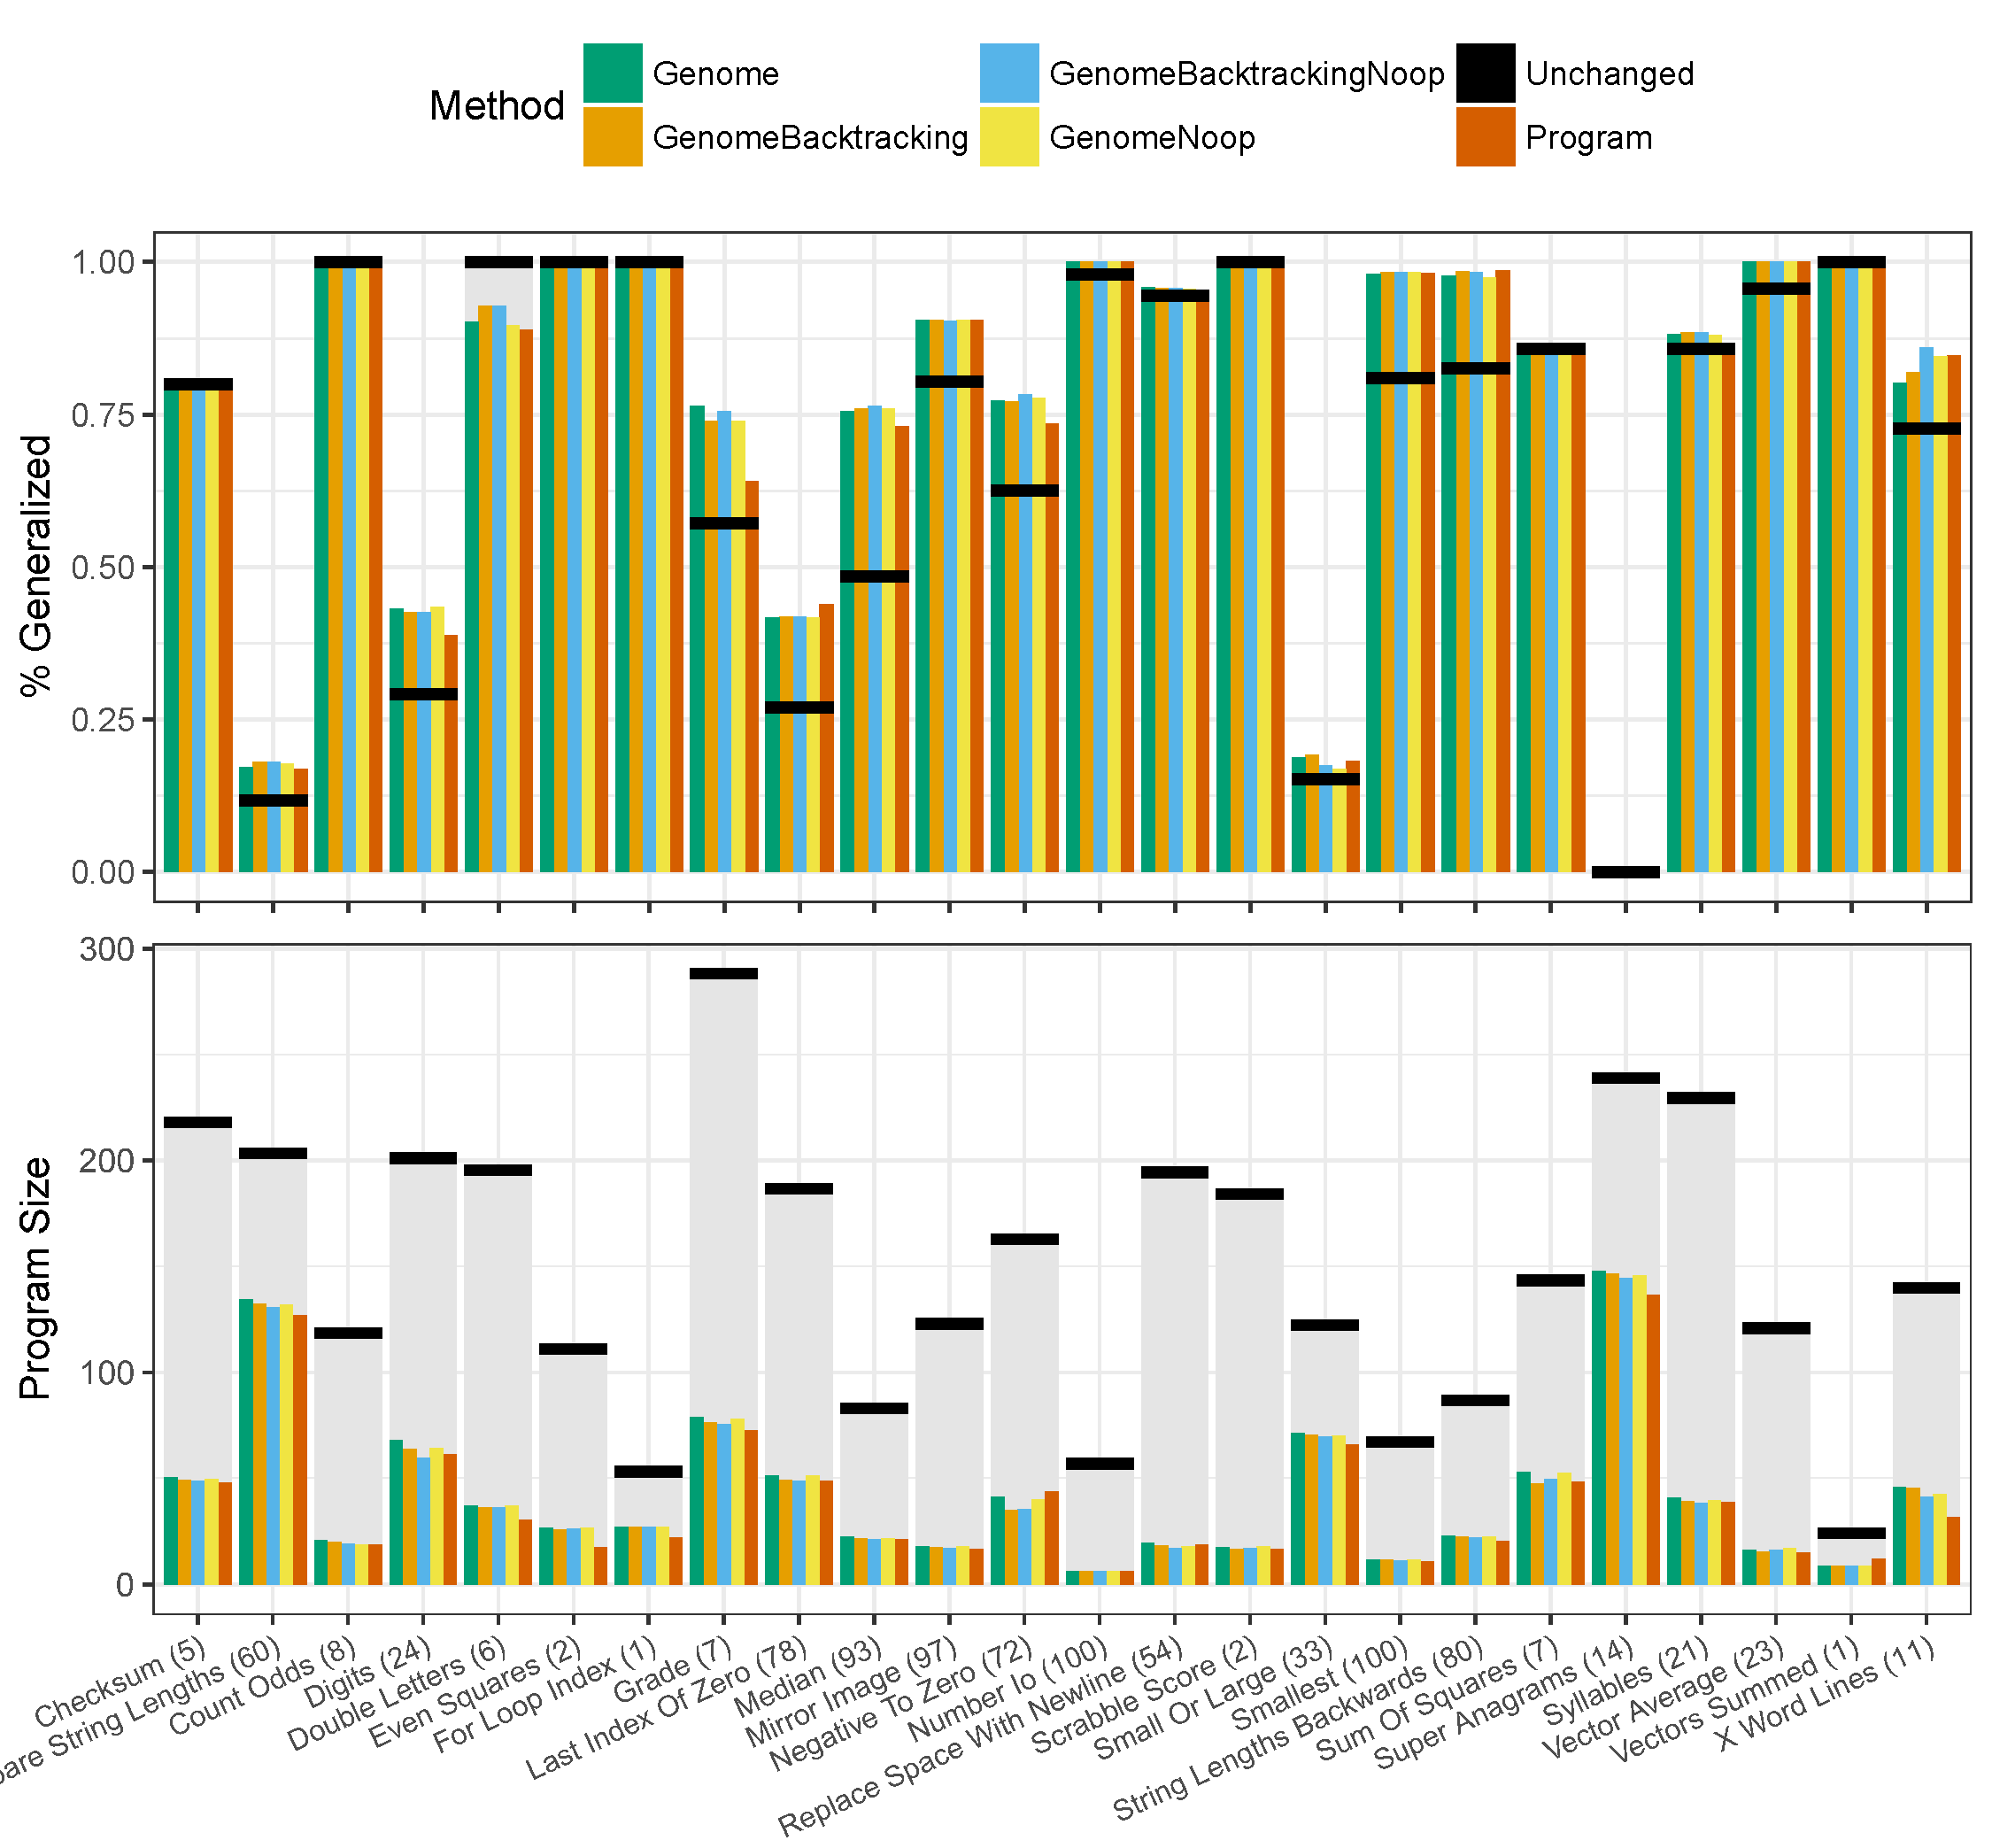
\includegraphics[width=1.0\textwidth]{stacked-bar}
 % \linewidth
\caption{The average program size of simplified programs and proportion
    of simplified programs that generalize to unseen test data of
    programs produced by our five
    simplification methods for each problem; the unchanged solution
    program averages are represented with horizontal black bars.
    Each simplification method performs repeated trials 
	using the same set of unchanged programs, and therefore has 
	the same opportunities for simplification as the other methods.
    The number of unchanged solution programs taken into account for each problem
    is given in parentheses, representing the number of starting points for each problem.}
\label{fig:bar:all}
\end{figure*}

% \begin{figure*}[h] %[t] sets the image at the top of the page; t = top, b = bottom, h = here%
% \centering
% 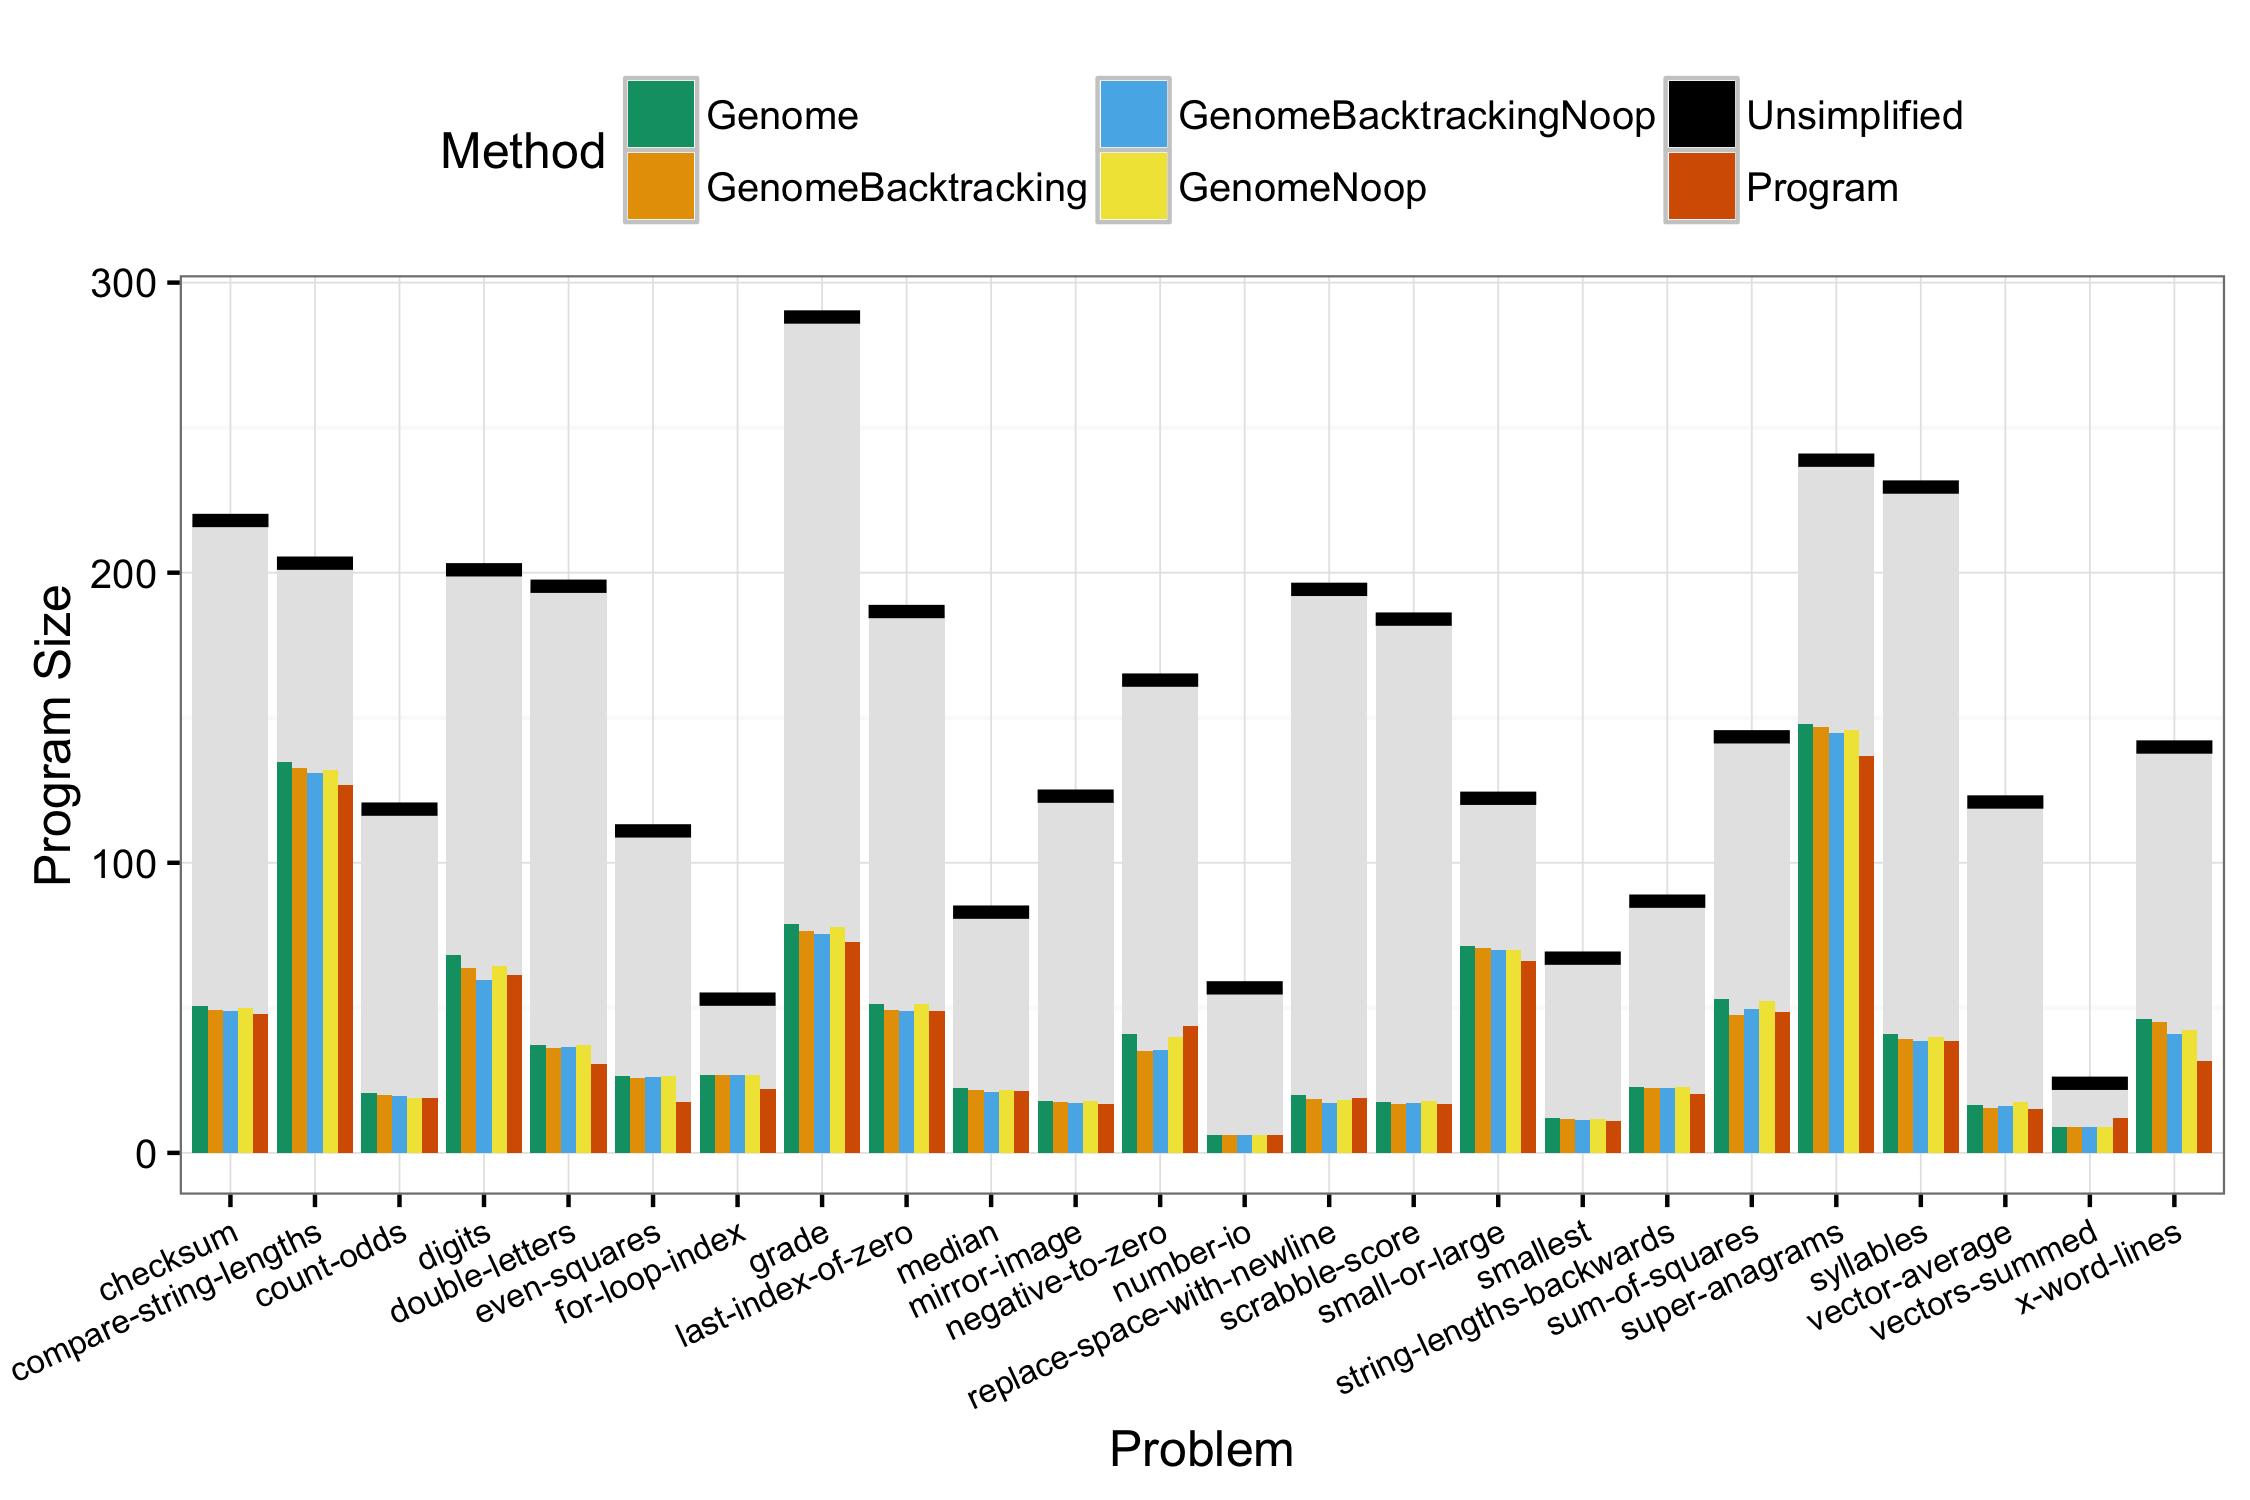
\includegraphics[width=0.89\textwidth]{Problem_by_Size_bar}
% %{stacked-bar}
%  % \linewidth
% \caption{The average program size of programs produced by our five 
% 	simplification methods for each problem set; the average program 
% 	sizes of the unchanged solution programs are represented with black 
% 	horizontal bars. Each simplification method performs repeated trials 
% 	using the same set of unchanged programs, and therefore has 
% 	the same opportunities for simplification as the other methods.
%     The number of unchanged solution programs taken into account for each problem
%     is given in parentheses, representing the number of starting points for each problem.}
% \label{fig:bar:size}
% \end{figure*}

% \begin{figure*}[h] %[t] sets the image at the top of the page; t = top, b = bottom, h = here%
% \centering
% 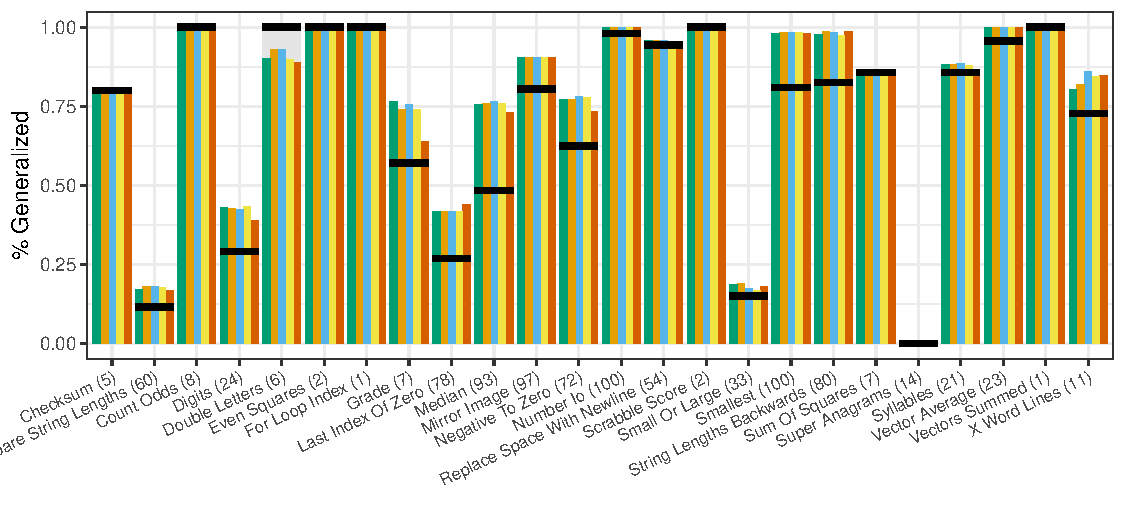
\includegraphics[width=0.89\textwidth]{Problem_by_PcntGen_bar_no_legend} % \linewidth
% \caption{The proportion of simplified programs that generalize to unseen test data
% 	for each problem, with the proportion of unchanged programs that generalize 
% 	indicated with black horizontal bars.
%     The number of unchanged solution programs taken into account for each problem
%     is given in parentheses, representing the number of starting points for each problem.
% % \hl{Question: In this figure, how much of the time are the simplified programs significantly better at generalization than the unsimplified programs? How would we measure this? Do we need to?}}
% % \hl{Is this just a bunch of \texttt{prop.test} in R, or am I not understanding
% % 	the question?
% }
% \label{fig:bar:percent_generalization}
% \end{figure*}


%\hl{Question: Should we somehow indicate the number of data points that go into each problem? Some problems have a lot of unchanged solutions ($>$ 90), and some have very few ($<$ 10), with the latter group potentially being small sample size, and the former group having more effect on the aggregate plots across problems.}
%\todo[inline]{It took me a while to figure out the question, but the 
%	later comment about DL only having 6 solutions to work with caused the 
%	light bulb to go off. I suspect we should indicate this somewhere. A table 
%	would be big. Maybe putting the number of initial successes in parens after 
%	the problem name in the axis labels? -- Nic}

We first consider the question of how much effect simplification has on the size of each solution program. Figure~\ref{fig:bar:all}a presents the average program size of the unchanged solution programs on each problem as a horizontal black line. It then gives the average simplified size of the simplified solution programs, with 100 trials per solution, for each of our five simplification methods. It is immediately clear that every simplification method has a large impact on the average size of the solution programs, with most shrinking to half their original size or smaller. 
In fact, the size
differences resulting from the various simplification methods are all 
quite small when compared to the difference between the simplified sizes
and the unchanged programs' sizes.

\begin{table}[t]
	\centering
	\caption{The average rank in size for each simplification method across the data in Figure~\ref{fig:bar:all}a, where lower rank means smaller programs. ``Unchanged'' is the rank of the evolved programs without any simplification.}
	\label{table:size-ranks}
	\begin{tabu} to \textwidth {l r}
		\toprule
		\textbf{Method} & \textbf{Average Rank} \\
		\midrule
		\textbf{Program} & 1.87 \\
		\textbf{Genome-Backtracking-Noop} & 2.13 \\
		\textbf{Genome-Backtracking} & 2.79 \\
		\textbf{Genome-Noop} & 3.60 \\
		\textbf{Genome} & 4.60 \\
		\textbf{Unchanged} & 6.00 \\
		\bottomrule
	\end{tabu}
\end{table}


In Table~\ref{table:size-ranks} we examine aggregate performance of each simplification method by calculating the average rank of program size for each method across the 24 problems, with rank 1 indicating the smallest average program size and rank 6 having largest.
%To examine aggregate performance of each simplification method, in Table~\ref{table:size-ranks} we calculate the average rank of program size for each method across the 24 problems, with rank 1 indicating the smallest average program size and rank 6 having largest.
Note that we include the unchanged programs as one ``method'', which is why we have 6 possible ranks. Program simplification achieves the smallest programs on average, with both of the Genome backtracking methods coming soon after. The genome methods without backtracking have worse average ranks, with the unchanged programs always having worst rank. Since parentheses are counted as part of the size of a program, and since the Genome methods cannot remove extraneous parentheses (as mentioned in Section~\ref{sec:simplification}), we hypothesize that Program simplification is able to achieve smaller sizes largely based on removing such parentheses.

The Friedman test on the data in Table~\ref{table:size-ranks} gives a \textit{p}-value $< 0.001$, indicating that at least one method performs significantly differently from the others. We then use a post-hoc Wilcoxon-Nemenyi-McDonald-Thompson test \cite{hollander1999nonparametric} to give the significance in the differences in ranking between each pair of methods at the $0.05$ significance level. Every simplification method besides Genome significantly outranks the Unchanged programs. Program also outranks Genome-Noop and Genome; and both Genome backtracking methods outrank Genome. Note that even though these results show significant differences in rank among the methods, most of the actual differences in average size are relatively small compared to the sizes of the unchanged programs.

%Program - none                              3.685940e-14
%GenomeBacktrackingNoop - none               6.733392e-12
%GenomeBacktracking - none                   1.343098e-08
%Program - Genome                            4.483262e-06
%GenomeBacktrackingNoop - Genome             4.216509e-05
%GenomeNoop - none                           9.320840e-05
%GenomeBacktracking - Genome                 8.811779e-03
%Program - GenomeNoop                        1.506233e-02
%---------------------------------------------------------
%  Cutoff for p-value of 0.05 or less (above)
%---------------------------------------------------------
%GenomeNoop - GenomeBacktrackingNoop         6.179964e-02
%Genome - none                               9.284012e-02
%GenomeNoop - Genome                         4.175994e-01
%Program - GenomeBacktracking                5.190458e-01
%GenomeNoop - GenomeBacktracking             6.489706e-01
%GenomeBacktrackingNoop - GenomeBacktracking 8.119145e-01
%Program - GenomeBacktrackingNoop            9.971909e-01

Next, we consider the effect of simplification on the generalization of programs to unseen test data. In Figure~\ref{fig:bar:all}b, we plot the percent of programs that generalize for each simplification method, as well as a horizontal bar representing the percent of unchanged programs that generalize.
Every simplification method either improves generalization or has no effect on every problem besides Double Letters.
%\footnote{The Double Letters problem has one of the smaller sample sizes of our data set, with only six solution programs as starting points. All six solutions generalize before simplification. Five of the six generalize most of the time after simplification, but one solution program has many simplifications that don't generalize.}
 Some of the increases in generalization appear substantial, 
improving as much as 25\% in the case of Median.

Also note that the five problems with the worst generalization in Figure~\ref{fig:bar:all}b are among the problems for which program sizes were largest in Figure~\ref{fig:bar:all}a. For whatever reason, programs that solve these problems tend to be large and unable to shrink, and do not generalize well. We hypothesize that large programs such as these contain many ad-hoc components that overfit to individual test cases without really ``learning'' the underlying program structure, and therefore do not generalize to unseen data.

%This supports our hypothesis that programs that are smaller but behaviorally identical on the training set tend to generalize better.

As with average program sizes, there do not appear to be large differences between the simplification methods in terms of generalization. To see if the small differences do affect rank, we calculated the average rank of each method across all problems. Here, rank 1 signifies the best (highest) generalization, and rank 6 represents the worst generalization. These average ranks are presented in Table~\ref{table:generalization-ranks}.

\begin{table}[t]
	\centering
	\caption{The average rank in generalization for each simplification method across the problems in Figure~\ref{fig:bar:all}b, where lower rank means better generalization. ``Unchanged'' is the rank of the evolved programs without any simplification.}
	\label{table:generalization-ranks}
	\begin{tabu} to \textwidth {l r}
		\toprule
		\textbf{Method} & \textbf{Average Rank} \\
		\midrule
		\textbf{Genome-Backtracking-Noop} & 2.73 \\
		\textbf{Genome-Backtracking} & 3.02 \\
		\textbf{Genome-Noop} & 3.29 \\
		\textbf{Genome} & 3.33 \\
		\textbf{Program} & 3.67 \\
		\textbf{Unchanged} & 4.96 \\
		\bottomrule
	\end{tabu}
\end{table}

For generalization, the differences in rank for the simplification methods are not as pronounced as with simplified sizes. Note that Program simplification, while producing the smallest programs, has the worst generalization of the simplification methods; all of the Genome-based methods remain in the same order. The Friedman test on the data in Table~\ref{table:generalization-ranks} gives a \textit{p}-value $< 0.001$, indicating that at least one method performs significantly differently from the others. We then use a post-hoc Wilcoxon-Nemenyi-McDonald-Thompson test \cite{hollander1999nonparametric} to give the significance in the differences in ranking between each pair of methods at the $0.05$ significance level. Here, every simplification method significantly outranks Unchanged. But, there is not a significant difference in generalization rank between any of the simplification methods. Thus the average rank of each method is approximately the same, which is unsurprising considering their similarities in Figure~\ref{fig:bar:all}b.

%GenomeBacktrackingNoop - none               1.532704e-06
%GenomeBacktracking - none                   8.164085e-05
%GenomeNoop - none                           1.186298e-03
%Genome - none                               1.892900e-03
%Program - none                              2.829973e-02
%%---------------------------------------------------------
%%  Cutoff for p-value of 0.05 or less (above)
%%---------------------------------------------------------
%Program - GenomeBacktrackingNoop            2.338544e-01
%Program - GenomeBacktracking                6.504160e-01
%GenomeNoop - GenomeBacktrackingNoop         7.712306e-01
%GenomeBacktrackingNoop - Genome             7.129661e-01
%GenomeBacktracking - Genome                 9.774709e-01
%GenomeNoop - Genome                         9.999987e-01
%Program - Genome                            9.701077e-01
%GenomeBacktrackingNoop - GenomeBacktracking 9.834383e-01
%GenomeNoop - GenomeBacktracking             9.881573e-01
%Program - GenomeNoop                        9.505945e-01


\begin{figure}[t] %[t] sets the image at the top of the page; t = top, b = bottom, h = here%
\centering
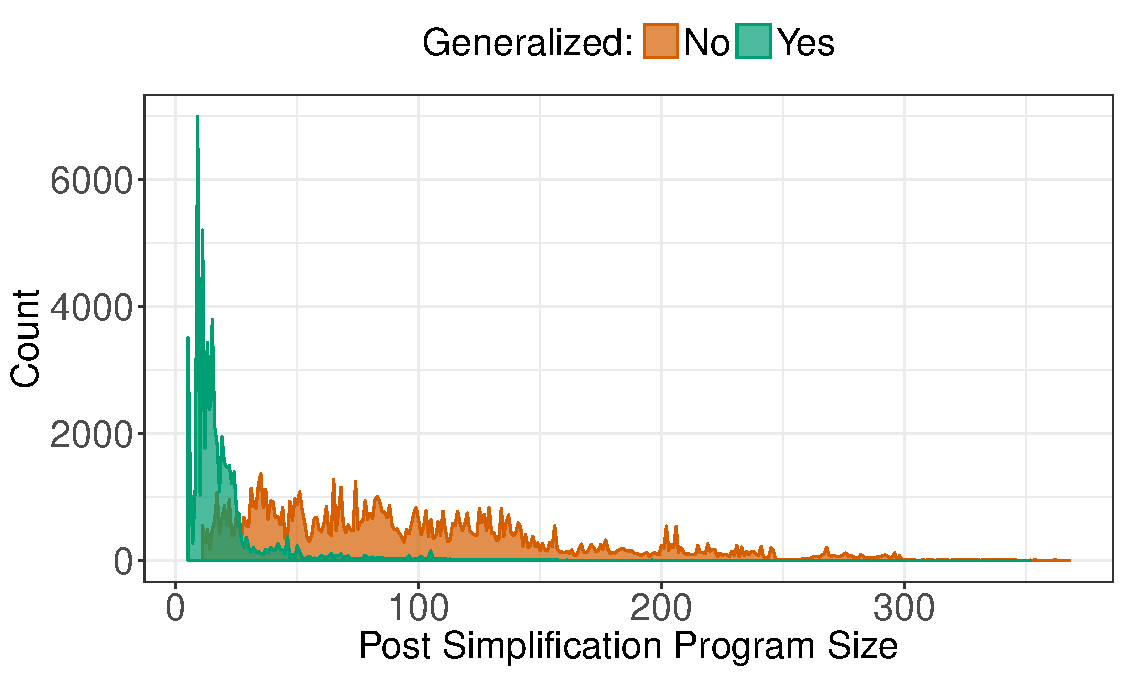
\includegraphics[width=\linewidth]{Size_Density_final}
%{Size_density_by_generalized_B_no_facet_count}
%{quad_density_new_bad}
\caption{We plot the counts of each post-simplification program size for cases where the unchanged program did \underline{not} generalize. Green (false) are programs that continued to not generalize after simplification; yellow (true) are programs that do generalize after simplification. The programs here correspond to the top row in Table~\ref{table:total-counts}.}
\label{fig:count:quad}
\end{figure}

\begin{table}[t]
	\centering
	\caption{This table records every single simplified program across all problems. The top row corresponds to unchanged programs that did not generalize, where the bottom row is those that did generalize. The left column contains all simplified programs that did not generalize, and the right column has those that did. For example, we see that there are 53787 simplified programs that generalize coming from original programs that did not generalize.}
	\label{table:total-counts}
	\begin{tabu} to \textwidth {l r r}
		\toprule
		& \multicolumn{2}{p{2.8cm}}{\textbf{Generalizes \newline Post-Simplification}} \\
		& \textbf{No} & \textbf{Yes} \\
		\midrule
		\textbf{Generalizes Pre: No} & 102,617 & 53,787 \\
		\textbf{Generalizes Pre: Yes} & 3,735  & 289,265 \\
		\bottomrule
	\end{tabu}
\end{table}


%\begin{figure}[t] %[t] sets the image at the top of the page; t = top, b = bottom, h = here%
%\centering
%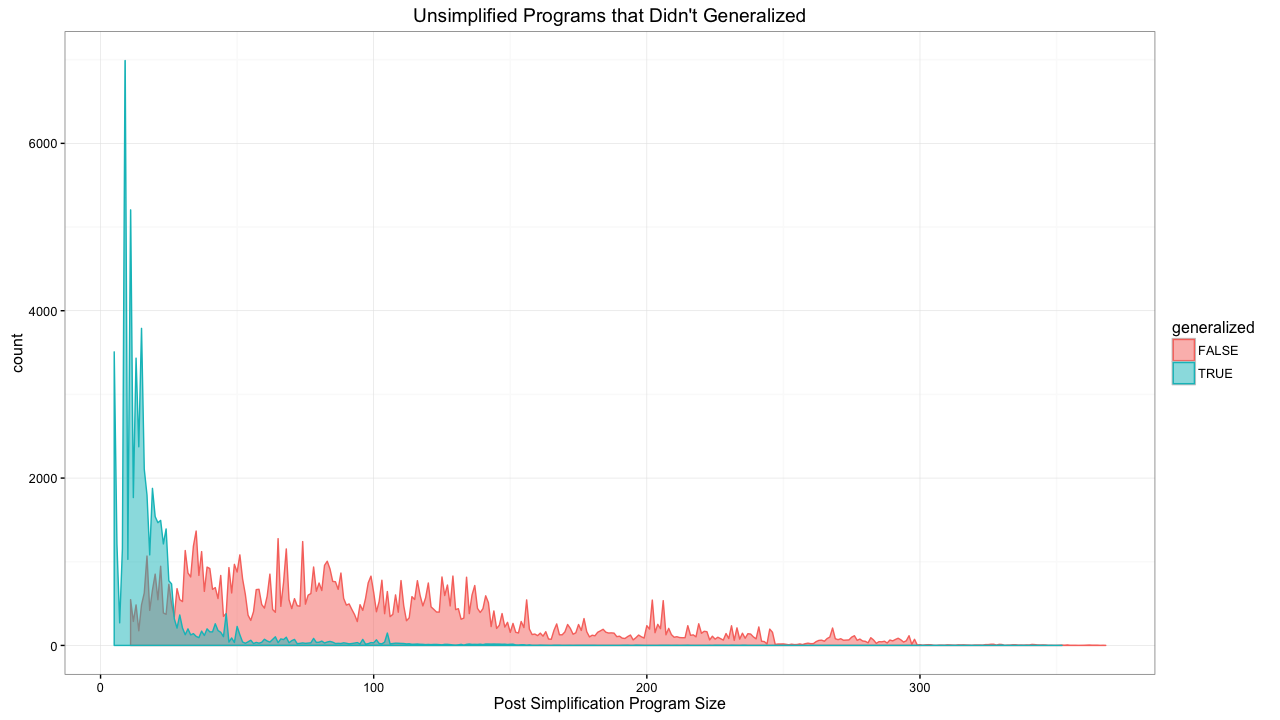
\includegraphics[width=\linewidth]{Size_density_by_generalized_B_no_facet_count}
%\caption{Size counts of simplified programs where pre-simplified program did \underline{not} generalize.}
%\label{fig:count:pre-simp-gen-false}
%\end{figure}
%
%\begin{figure}[t] %[t] sets the image at the top of the page; t = top, b = bottom, h = here%
%\centering
%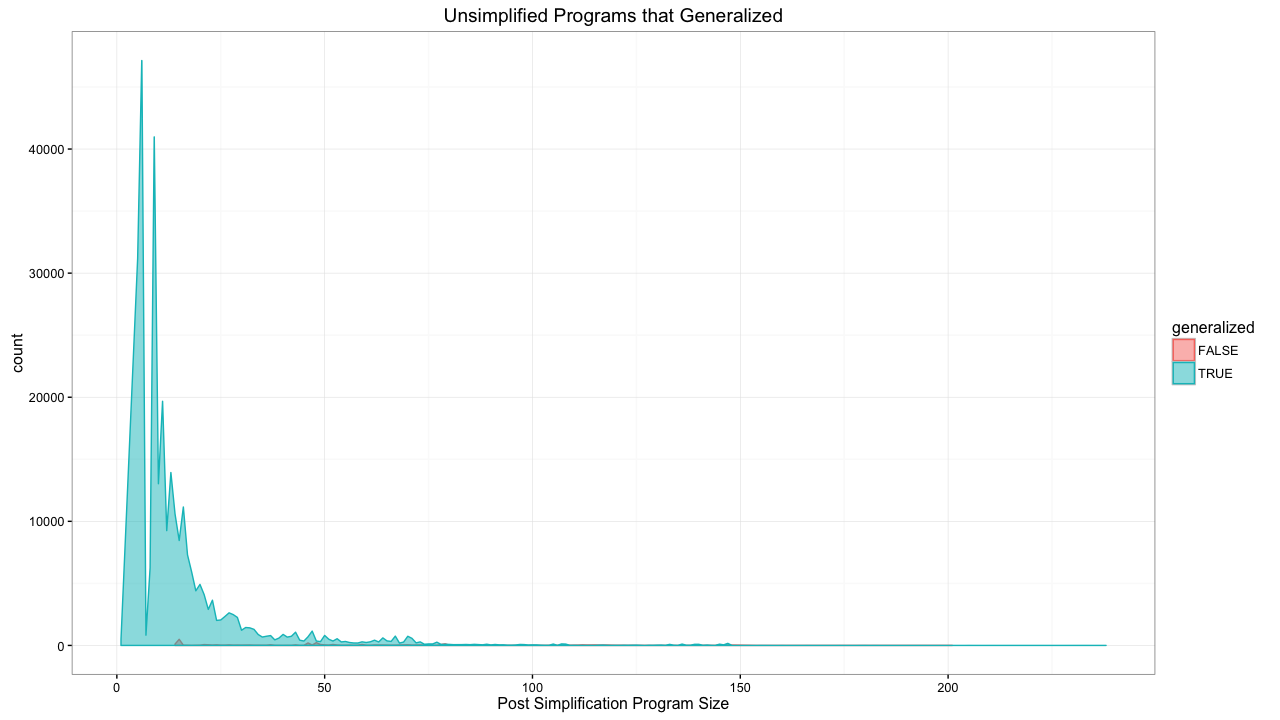
\includegraphics[width=\linewidth]{Size_density_by_generalized_A_no_facet_count}
%\caption{Size counts of simplified programs where pre-simplified program did generalize.}
%\label{fig:count:pre-simp-gen-true}
%\end{figure}

\hl{NEED to make this refer to the new table.}
Ignoring the lines for now, the numbers in Figure~\ref{fig:count:quad} give the total count of each combination of programs that did/did not generalize pre-simplification with  did/did not generalize post-simplification. Considering the top row of evolved programs that did not generalize, over 33\% generalized after simplification. On the other hand, out of the starting programs that did generalize before simplification (the bottom row), only about 1.2\% of the simplifications broke them so that they did not generalize. This gives strong evidence that simplification can be used to make evolved programs more likely to generalize, without a large risk of breaking programs that already generalize. In total, 65\% of the unchanged programs generalized before simplification; that number rises to 76\% after simplification, an increase in generalization of 11 percentage points.

% Pre:  (3735 + 289265) / (102617 + 53787 + 3735 + 289265) = .652
% Post: (53787 + 289265) / (102617 + 53787 + 3735 + 289265) = .763

We next want to explore how size after simplification corresponds to the generalization of simplified programs. The lines in Figure \ref{fig:count:quad} plot the counts of the sizes of the simplified programs for the same four sets of programs, aggregated across all problems. The top row only includes those simplifications that started with unchanged programs that did not generalize. These two subplots clearly show that when the resulting simplified program was relatively small (with size less than about 25), it was much more likely to change from ungeneralizing to generalizing, as seen in the upper-right plot. On the other hand, programs that remained larger after simplification were more likely to remain ungeneralizing, shown in the upper-left plot. Thus, most of the improvements in generalization that we described previously come from simplified programs that achieve small sizes. This clearly shows that there is a correlation, if not causation, between post-simplification size and the probability of generalization.

The bottom two plots in Figure~\ref{fig:count:quad} also give the counts of sizes of the simplified programs, but this time for those unchanged programs that did generalize. First, note that the scale of the $y$-axis is over 5 times as large as for the top row; as we saw previously, about twice as many unchanged programs generalized as those that did not. We see that generalizing programs tended to be very small here as well.


%%%%%%% KEEP THE FOLLOWING IF WE HAVE SPACE

%The correlation between post-simplification size and generalization can also be seen in Figure~\ref{fig:nic-plot}. Here, each point represents one simplified program; which plot it belongs to depends on whether it generalized before or after simplification, with the same configuration as Figure~\ref{fig:count:quad}. The $x$-axis gives pre-simplification size of the program, and the $y$-axis gives simplified program size; thus, every point must lie under the $y = x$ line. Points close to the $y = x$ line did not reduce much during simplification; those further below the $y = x$ line correspond to those that shrank more.
%
%\begin{figure}[t] %[t] sets the image at the top of the page; t = top, b = bottom, h = here%
%\centering
%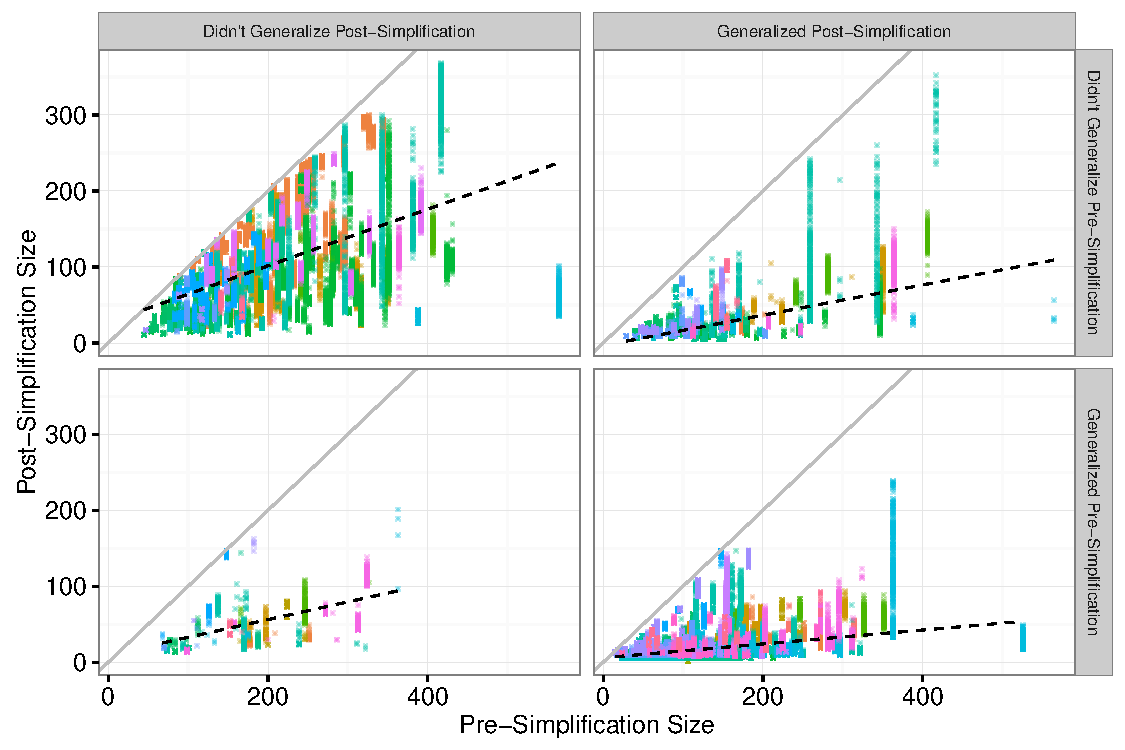
\includegraphics[width=\linewidth]{Quad_Scatter} % \linewidth
%\caption{In each of the subgraphs, a simplified program is plotted at each point, with its pre-simplified size on the $x$-axis and its post-simplified size on the $y$-axis. Vertical striping is the result of simplifying each unchanged program 100 times for each of the 5 simplification methods. The top two plots contain programs that did not generalze pre-simplification, and the bottom two plots contain programs that did generalize pre-simplification. The left two plots are simplified programs that do not generalize; the right plots do generalize. For each plot, we also give a linear trend line.}
%\label{fig:nic-plot}
%\end{figure}
%
%In each plot we draw a linear fit line showing the relationship of unchanged size and simplified size. In the plots in the left column, in which simplified programs did not generalize, the slope is considerably higher than in the right column plots where the simplified programs do generalize. This gives further confirmation that programs that shrink considerably from their original sizes are more likely to generalize.


%\begin{figure}[t] %[t] sets the image at the top of the page; t = top, b = bottom, h = here%
%\centering
%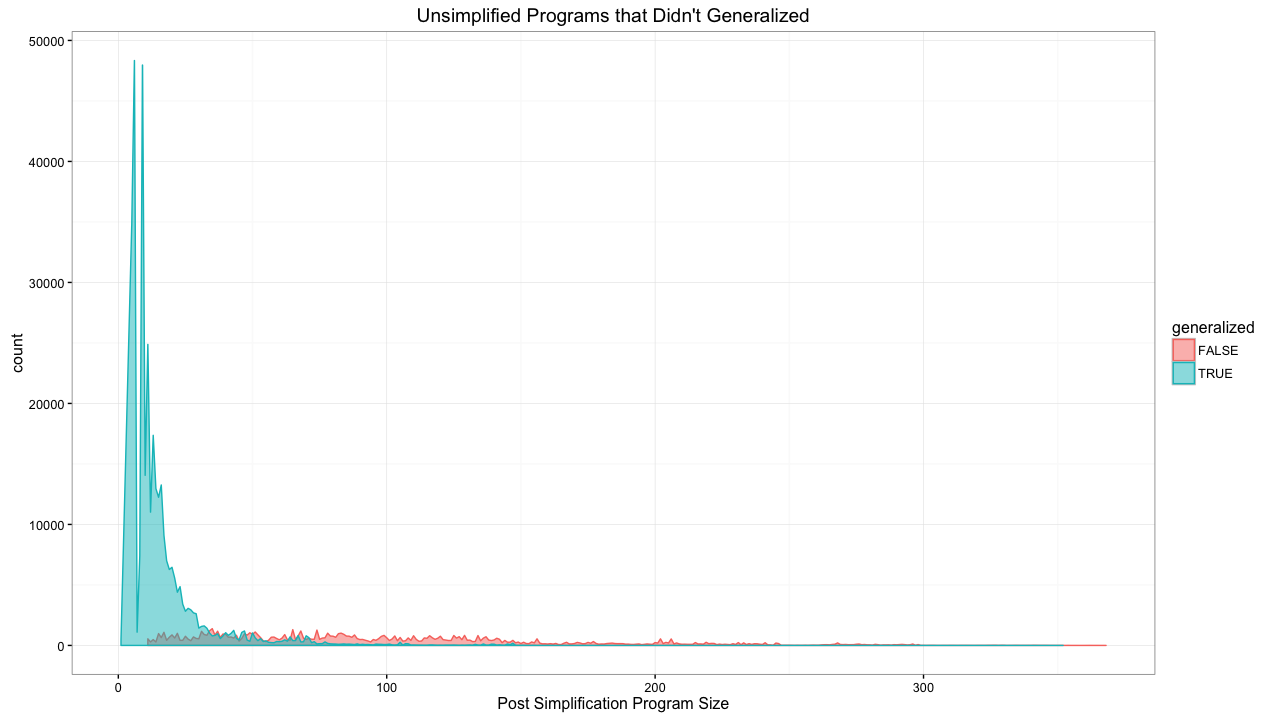
\includegraphics[width=\linewidth]{Size_density_by_generalized_count}
%\caption{Size counts of simplified programs. Includes all simplified programs, from both ones that did and did not generalize pre-simplification.}
%\label{fig:count:gen}
%\end{figure}

%These look at the same graphs, but faceted.
%
%\begin{figure}[t] %[t] sets the image at the top of the page; t = top, b = bottom, h = here%
%\centering
%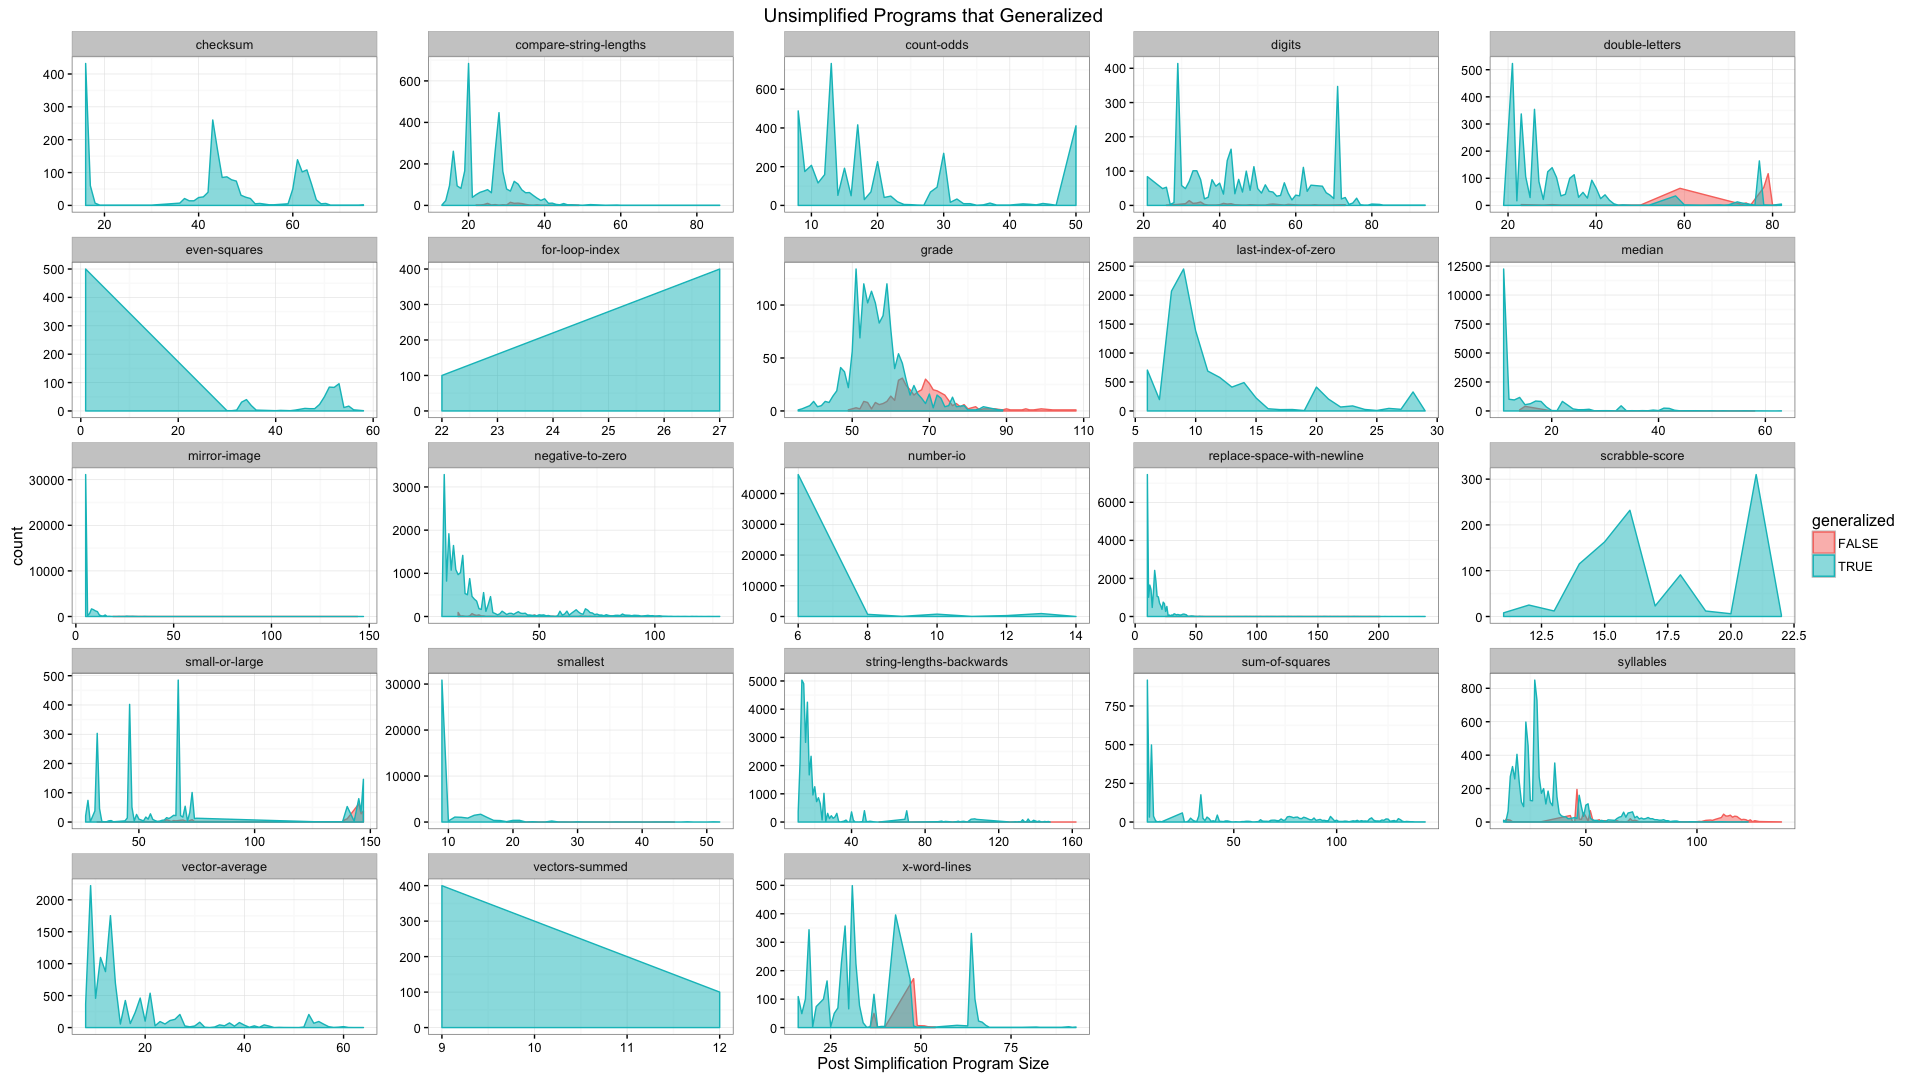
\includegraphics[width=\linewidth]{Size_density_by_generalized_A_count}
%\caption{Size counts of simplified programs where pre-simplified program did generalize.}
%\label{fig:count:pre-simp-gen-true}
%\end{figure}
%
%\begin{figure}[t] %[t] sets the image at the top of the page; t = top, b = bottom, h = here%
%\centering
%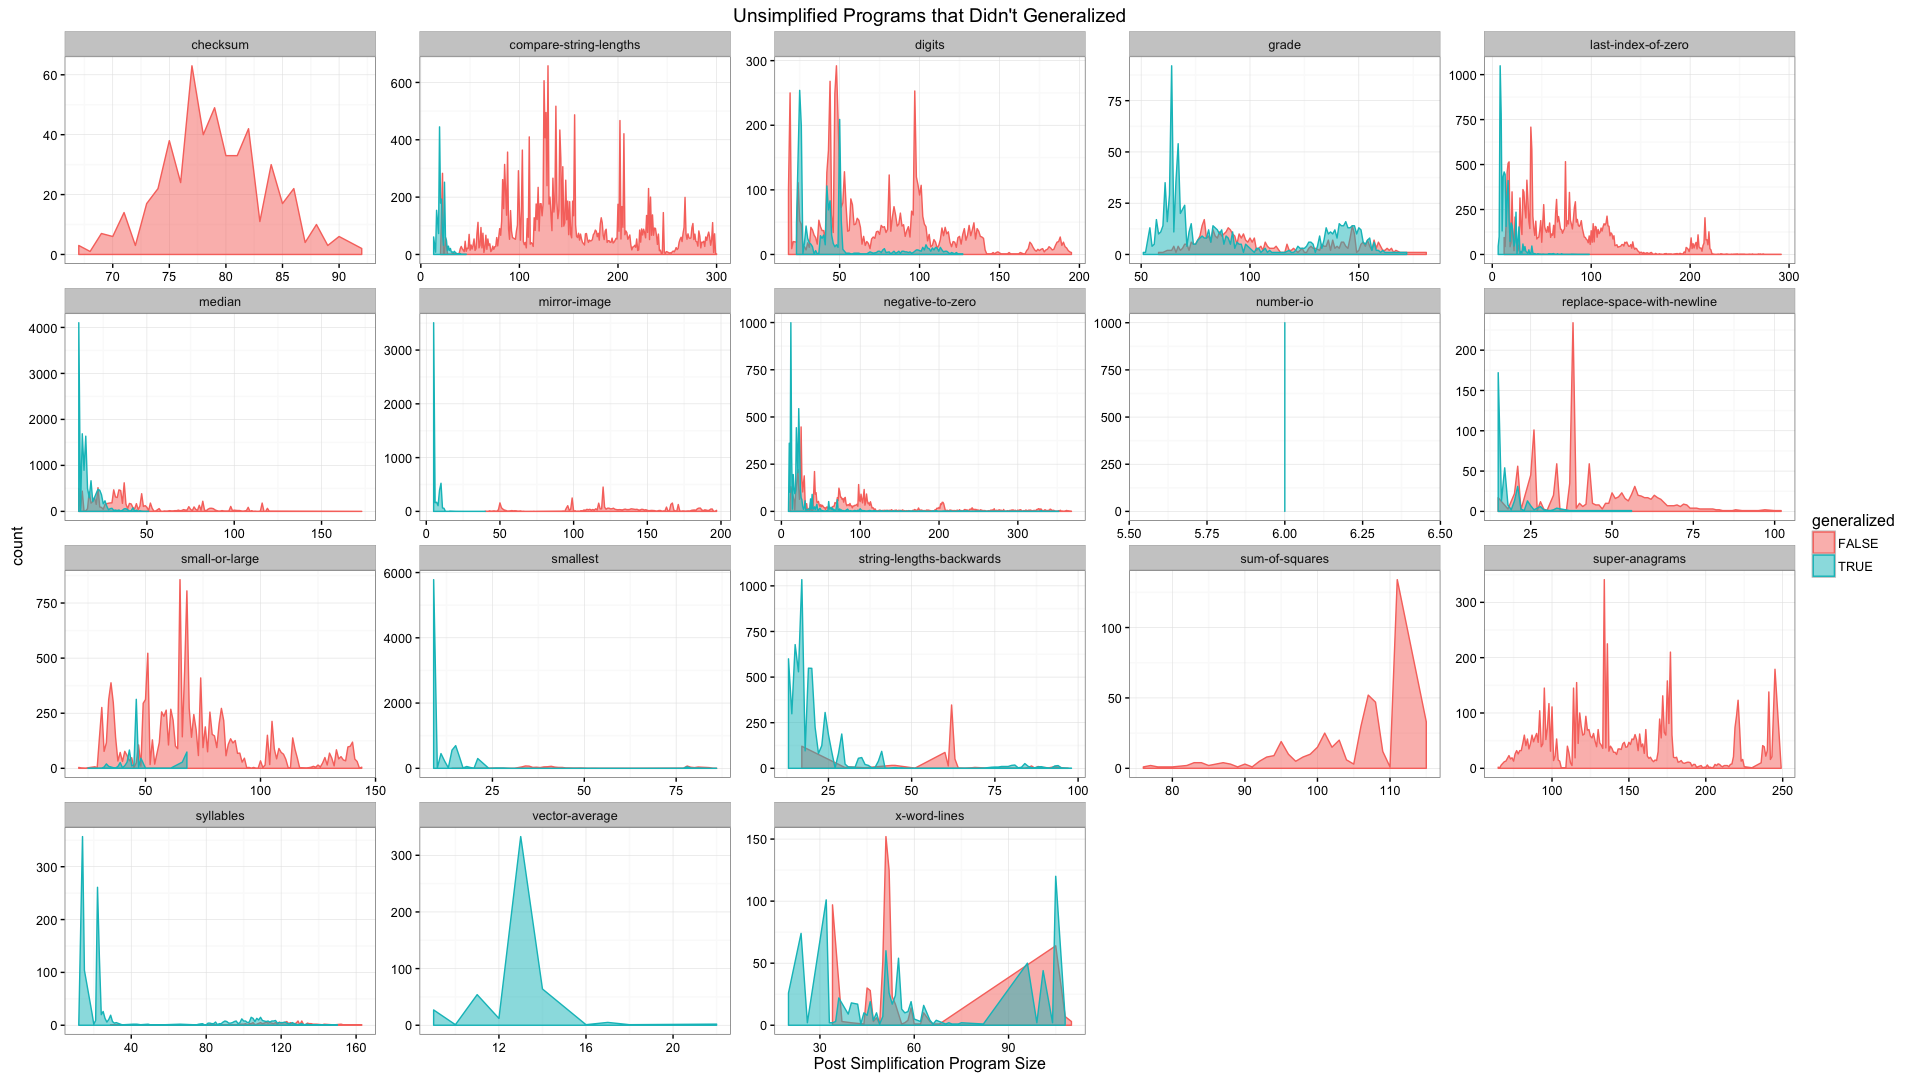
\includegraphics[width=\linewidth]{Size_density_by_generalized_B_count}
%\caption{Size counts of simplified programs where pre-simplified program did \underline{not} generalize.}
%\label{fig:count:pre-simp-gen-true}
%\end{figure}


\section{Discussion}
\label{sec:discussion}

%Here are some potentially interesting questions to explore with this data:
%
%    Which simplification method tends to result in the smallest programs on average? Is there any significant differences here?
%
%    Is getting smaller during simplification important for generalization? In other words, do smaller programs post-simplification tend to generalize better than larger ones?
%
%        Note: we could ask this question of all the simplified programs, but we could also concentrate only on runs that had some generalizing programs and some non-generalizing programs, which might give us a more detailed view. It would probably be worthwhile to look into both of these. I'm not sure exactly how we would investigate this. @mcphee made some cool graphs last year that start answering this question. I've included one at the bottom of this post that was made with limited data; a similar graph for the full data might be a good place to start.
%
%    It might be worthwhile to break this big plot into smaller plots, grouping together similar plots. For example, we might group plots based on how often unsimplified programs generalize -- groups of something like 0-50\%, 50-95\%, and 95-100\% generalization. Or, we could do it some other way. But, this could definitely help with spotting differences based on problem.
%

%\hl{    Would a multi-restart simplification get us to smaller programs more often than the other methods we've tried? This could potentially avoid unlucky local minima. The backtracking methods are also trying to avoid unlucky local minima, so this would be an interesting comparison. It seems like we could answer this question with the data we have.}
%
%\todo[inline]{I don't really see how we could answer that question with
%this data? It's definitely a cool question, but seems more future work
%than this paper. -- Nic}

As noted earlier, all five simplification methods lead to substantial
reductions in program size across all 24 test problems, as shown in
Figure~\ref{fig:bar:all}a, with the average simplified sizes often 
well under half the original sizes, and sometimes much smaller than that.

Further, all the simplification methods improved generalization rates for
all but a few problems (see Figure~\ref{fig:bar:all}b),
but again with little difference among the simplification methods.
In some cases, e.g., Count Odds, all the unsimplified programs already
generalized, so the best simplification could do is to not make things
worse. In other cases, such as
Checksum, Double Letters, and Vectors Summed, there were very few 
solution programs generated in the initial 100 PushGP runs (5, 6, and 1,
respectively). With so few data points to work with it's not surprising
that in some cases (e.g., Checksum and Vectors Summed) there was no change
in generalization. In the case of Double Letters, five of the six initial
solutions were consistently simplified without affecting generalization.
The sixth solution, however, frequently led to simplifications that no 
longer generalized. Only 37 of the 100 Program simplification results, 
for example, generalized, while only 45 of the 100 Genome simplifications
generalized.

%\todo[inline]{All the the failures I've looked at (and I looked at quite a
%	few) have a total error of 6, with errors of 2 on the same three test
%	cases. They all share a weird sequence of 20 `!' characters in a row
%	early in their simplified programs, which smells really fragile to me,
%	but I haven't dug into the programs enough to know if that's the issue.}

Our attempts at improving on simplification of Push programs by simplifying genomes, including with backtracking and NOOPs, seems mostly for naught. Program simplification led to the smallest programs, though as mentioned, this might be due to its ability to remove extraneous parentheses as opposed to potentially overfit code. On the other hand, Genome-Backtracking-Noop simplification had the best rank on generalization, though not significantly so, and had the second smallest rank on simplified size of programs. The backtracking ability of this method may have allowed it to avoid some locally optimal programs. We have anecdotally noticed an example where Program simplification is not able to escape such a local optima, and Genome-Backtracking-Noop might have made improvements in such cases. Adding NOOPs seems to have a lesser effect, since the Genome-Noop method produced larger programs than Genome-Backtracking, yet both were smaller than Genome without either enhancement.

Despite all of these minor differences, all simplification methods performed rather similarly across the board, with all showing major improvements over not using simplification. Thus, the choice of using any simplification method seems like the more significant decision than which simplification method to use.


Figure~\ref{fig:count:quad} makes it clear that
smaller post-simplification sizes were strongly correlated with the
ability to generalize after simplification. This is consistent with 
a broad range of work that either argues theoretically (e.g., the minimum
description length principle~\cite{iba1994genetic, zhang1995balancing}) 
and/or empirically
that smaller programs will be more likely to generalize~\cite{rosca:1996:gVsGP}.
While there have been contrary results that show that program size and
generalization are not always correlated~\cite{silva2012operator}, the
correlation seems extremely strong in our data. 

The relationship between
program size and generalization is almost certainly driven at least in part
by both the problem being solved and the representation being used for
solutions. It's possible, therefore, that the strong correlation we see
is in some way related to the kinds of software synthesis problems we're using
as benchmarks, which clearly behave differently from other common application areas such as symbolic regression and classification. 
%It is also possible that the design decisions in PushGP play a role here.

It is also possible that the design decisions in PushGP play a role here. Any
attempt to control or reduce program size in GP is premised on the idea that
there must be some parts of the program that aren't playing an important role
and can thus be removed; such code has been called many things over the years,
such as ``introns'' or ``bloat''. The fact that the evolved PushGP solutions
were bigger than strictly necessary (often by a substantial margin) is arguably
not attributable to ``bloat'' as it's typically been 
understood~\cite{poli08:fieldguide}, since in PushGP we don't see a 
general tendency towards increasing program size over time. 
There is obviously ``unnecessary'' code in these evolved Push programs, but understanding the source and role of this removable Push 
code is complex, in part because there are potentially many categories 
of unused or unnecessary code
in Push.

% Examples include:
%\begin{itemize}
%	\item Instructions that do nothing because they require arguments 
%	that are not on the appropriate stacks when they are executed. 
%	\item Instructions that do \emph{something}, but not something that has an 
%	impact on the final result because, e.g., they act on values on stacks 
%	that play no role in the key computation. 
%	\item Instructions whose \emph{presence} is important (e.g., as a marker 
%	or to make sure the \texttt{exec} stack has the right depth), but 
%	whose details or \emph{behavior} is not.
%\end{itemize}
%Note also that the ``activity'' of many of these instructions is highly
%dependent on context. An instruction that does nothing in a parent because
%the arguments it needs aren't available, might play a prominent role in a
%child if a change ``upstream'' causes those arguments to now be available.
%
%These dynamics are very different from many tree-based GP systems, where
%changes in argument subtrees will change the \emph{value} computed at a 
%node, but won't typically change the \emph{semantics} of the operator at that
%node. A plus node in a tree will always do addition, even if changes in its
%arguments lead to different sums; the plus node will (in most tree-based
%systems) never simply fail to act because an argument is missing.
%
%So in the same way that the design of our simplification methods was
%tightly coupled to the details of Push and Plush, it would not be surprising
%if at least some of the results (e.g., the relationship between size and
%generalization) were also tied to the specifics of PushGP. One common
%anecdotal observation is that unsimplified evolved Push programs often
%contain large numbers of looping and recursion constructs that are removed
%in the simplification process. It's possible that in many cases these loops
%are performing ``unnecessary'' computation and counting on the PushGP
%execution limits to stop them and force the return of an answer. This sort
%of approach is likely to be quite brittle, and eliminating these unnecessary
%loops might be a source of improved generalization. All of which is rather
%deeply intertwined with key details of PushGP.




\section{Conclusions and Future Work}
\label{sec:conclusions}

The results of our experiments show, across a range of software synthesis benchmark problems, that smaller programs evolved byPushGP tend to generalize better than larger programs. The results also show that evolved programs can be automatically simplified using a variety of simple hill-climbing procedures, and that simplified programs tend to generalize better than unsimplified programs. Furthermore, programs that can be successfully simplified (that is, that the simplification procedure can make much smaller) are more likely to show improved generalization after simplification. The differences between our simplification methods were not significant, but significant improvements were produced when any of them was used.

The recommendation, therefore, for users of PushGP is to always perform automatic simplification on the results of evolution, using any of the methods described here. There is a reasonable chance that doing so will improve the generalization of evolved programs, and a much smaller chance that it will hurt it. If a program is substantially smaller after automatic simplification, then it will have an even better chance of generalizing.

Would the same advice apply to users of other types of GP systems? For some systems, such as tree-based GP with non-numeric functions, automatic simplification based on hill-climbing may be non-trival. Our methods might be applied more easily to other forms of GP, including grammatical evolution, Cartesian GP, and linear GP systems.

An extension of the work presented here would be to run the same tests using different types of problems, such as classification and symbolic regression. Another area for future work is to improve the automatic simplification methods themselves. While we presented results with several simplification methods, all of them used a simple hill-climbing search procedure that can get stuck in local minima, even when using backtracking steps. A multi-start hillclimber, for example, might simplify programs more reliably.


\begin{acks}
  
This material is based upon work supported by the National Science Foundation under Grants No. 1617087, 1129139 and 1331283. Any opinions, findings, and conclusions or recommendations expressed in this publication are those of the authors and do not necessarily reflect the views of the National Science Foundation.

\end{acks}
